\begin{frame}{interlude: editing disassembly format}
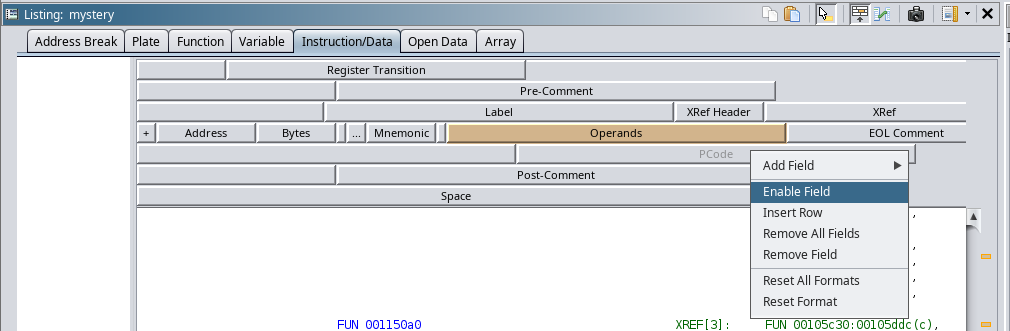
\includegraphics[width=\textwidth]{../re-tools/ghidra-enable-show-pcode}
\end{frame}

\begin{frame}{PCode}
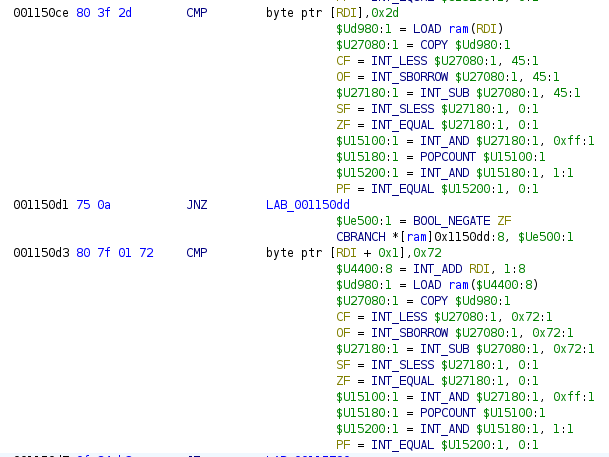
\includegraphics[height=0.9\textheight]{../re-tools/ghidra-pcode-ex}
\end{frame}

\begin{frame}{Intermediate Representations}
\begin{itemize}
\item Ghidra converts instructions to this PCode language
    \begin{itemize}
    \item describes effects of each instruction for other parts of Ghidra
    \item allows `easy' support for ARM, MIPS, \ldots
    \end{itemize}
\item function graph we saw using PCode information, probably
\item decompiler is basically a PCode to C compiler
    \begin{itemize}
    \item does the same kind of optimizations/etc. normal compiler does
    \item different output language
    \end{itemize}
\item Ghidra has `find similar functions' tool that probably uses this
\end{itemize}
\end{frame}


